\documentclass[11pt]{article}
\usepackage[utf8]{inputenc}
\usepackage{parskip}
\usepackage[a4paper, margin=1in]{geometry}
\usepackage{graphicx}
\usepackage{hyperref}
\usepackage{listings}
\usepackage{array}
\usepackage[capitalise,noabbrev]{cleveref}
\usepackage{rotating}

% Custom json syntax highlightning
\usepackage{bera}
\usepackage{xcolor}

\definecolor{background}{HTML}{EEEEEE}
 
\lstdefinestyle{mystyle}{
	basicstyle=\ttfamily\small,
	backgroundcolor=\color{background},
	breakatwhitespace=false,        
    frame=lines,   
    breaklines=true,                 
    captionpos=b,                    
    keepspaces=true,                 
    numbers=left,                    
    numbersep=5pt,                  
    showspaces=false,                
    showstringspaces=false,
    showtabs=false,                  
	tabsize=4,
	numbers=left,
	numberstyle=\tiny\color{black},
	numbersep=10pt,
	framexleftmargin=5pt,
	framexrightmargin=5pt,
}

\lstset{style=mystyle}

\definecolor{jsonstring}{RGB}{61,107,42}
\colorlet{jsonpunct}{red!60!black}
\definecolor{jsondelim}{RGB}{20,105,176}
\colorlet{jsonnumb}{magenta!60!black}

\lstdefinelanguage{json}{
	stringstyle={\color{jsonstring}},
	string = [d]{"},
    literate=
     *{0}{{{\color{jsonnumb}0}}}{1}
      {1}{{{\color{jsonnumb}1}}}{1}
      {2}{{{\color{jsonnumb}2}}}{1}
      {3}{{{\color{jsonnumb}3}}}{1}
      {4}{{{\color{jsonnumb}4}}}{1}
      {5}{{{\color{jsonnumb}5}}}{1}
      {6}{{{\color{jsonnumb}6}}}{1}
      {7}{{{\color{jsonnumb}7}}}{1}
      {8}{{{\color{jsonnumb}8}}}{1}
      {9}{{{\color{jsonnumb}9}}}{1}
      {:}{{{\color{jsonpunct}{:}}}}{1}
      {,}{{{\color{jsonpunct}{,}}}}{1}
      {\{}{{{\color{jsondelim}{\{}}}}{1}
      {\}}{{{\color{jsondelim}{\}}}}}{1}
      {[}{{{\color{jsondelim}{[}}}}{1}
      {]}{{{\color{jsondelim}{]}}}}{1},
}

\definecolor{javared}{rgb}{0.6,0,0} % for strings
\definecolor{javagreen}{rgb}{0.25,0.5,0.35} % comments
\definecolor{javapurple}{rgb}{0.5,0,0.35} % keywords
\definecolor{javadocblue}{rgb}{0.25,0.35,0.75} % javadoc
\definecolor{javablue}{HTML}{348B98}
 
\lstset{language=Java,
	keywordstyle=\color{javapurple}\bfseries,
	stringstyle=\color{javared},
	commentstyle=\color{javagreen},
	morecomment=[s][\color{javadocblue}]{/**}{*/},
	emph=[1]% Java Classes
    {%
		AggregateIterable,
		FindIterable,
        Document,
        Arrays,
        Aggregates,
        Accumulators,
        Bson,
        RuntimeException,
        User,
        Session,
        Movie,
        Adapter,
        Sorts,
        Projections,
    },
	emphstyle=[1]{\color{javablue}},
}

\renewcommand{\arraystretch}{1.5}

\title{Task 3 -- Movie Database\\ 
	\Large Design Document}
\date{\today}
\author{Federico Fregosi, Mirko Laruina,\\
        Riccardo Mancini, Gianmarco Petrelli}

\begin{document}
\pagenumbering{gobble}
\maketitle
\vfill
\setcounter{tocdepth}{2}
\tableofcontents
\vfill
\clearpage
\setcounter{page}{1}
\pagenumbering{arabic}

\section{Specifications}

\subsection{Existing Application Summary}
The application is an aggregator of movies and movie ratings with the purpose 
of providing logged users statistics and informations about a large set of movies.
Logged-in user can also rate movies they have watched while not logged-in users 
may still use the service to browse movie rankings and statistics but they are not
able to give their rate. Only movies released in Italy are considered.

All users can search a movie and view its details (e.g., title, original title, duration, 
cast, ...) along with its average rating from users and from external sources. 

In addition, all users can browse the list of movies sorting and filtering it by many parameters
(e.g. year, genre, country, actors, ...).

System administrators can view all user profile pages and ban users. In order to do that, he can 
check the full history of ratings. Once a user is banned, he can no longer log in and his username and email cannot be used by new users.

The movie database will be built upon the publicly available IMDb dataset.

The ratings will be gathered also by periodically scraping external websites 
(e.g., Rotten Tomatoes, Coming Soon, MyMovies).

\subsection{Task 3 additions overview}
Upon the application described above, which we have already designed and 
implemented, we will add the management of followed/following relationships 
between users and the suggestion of movies to the user based on his ratings.

In particular, every logged user can follow any other user and un-follow them 
later if they wish. Following another user gives the user the ability to see 
which movies the latter rates in a dedicated section. In this section the user 
will see all ratings from followed users in chronological order.
In his profile a user will see a new 
section from which he can browse his followed users
and the users that are following him and receive suggestions for new user to 
follow based on his current followed and following users. 
The search functionality will be extended to all registered user in order to 
more quickly find another user given his username.

Furthermore, in his homepage, a logged user will receive suggestions about 
movies that he might like based on his ratings and the most recent ratings on the platform. By doing so, suggestions will reflect the current trends.

\subsection{Actors}
Anonymous user, registered user, administrator and updater ``bot''.

\subsection{Requirement Analysis}

\subsubsection{Functional Requirements}
In addition to what has already been defined in Task2, a \textbf{registered user} can:
\begin{itemize}
	\item follow another registered user
	\item un-follow a followed users
	\item browse the users he is following
	\item browse the users that are following him
	\item browse suggestions for new users to follow
	\item browse a list of suggested movies
	\item browse the latest ratings of followed users
	\item view the profile page of any other user
	\item search a user through a query by username
\end{itemize}

\subsubsection{Non-Functional Requirements}
\begin{itemize}
	\item \textbf{Availability}: the Database must be replicated in order to be always available. Write operations on the Database can be eventually consistent.
	\item \textbf{Scalability}: the application must be able to scale to an arbitrary number of servers.
	\item \textbf{Security}: passwords must be stored in a secure way.
	\item \textbf{Responsive UI}: Client-side application must provide a responsive view both for pc, 
	laptops and mobile devices.
\end{itemize}

\section{Design}

\subsection{Use-case diagram}

\begin{sidewaysfigure}[h!]
    \centering
    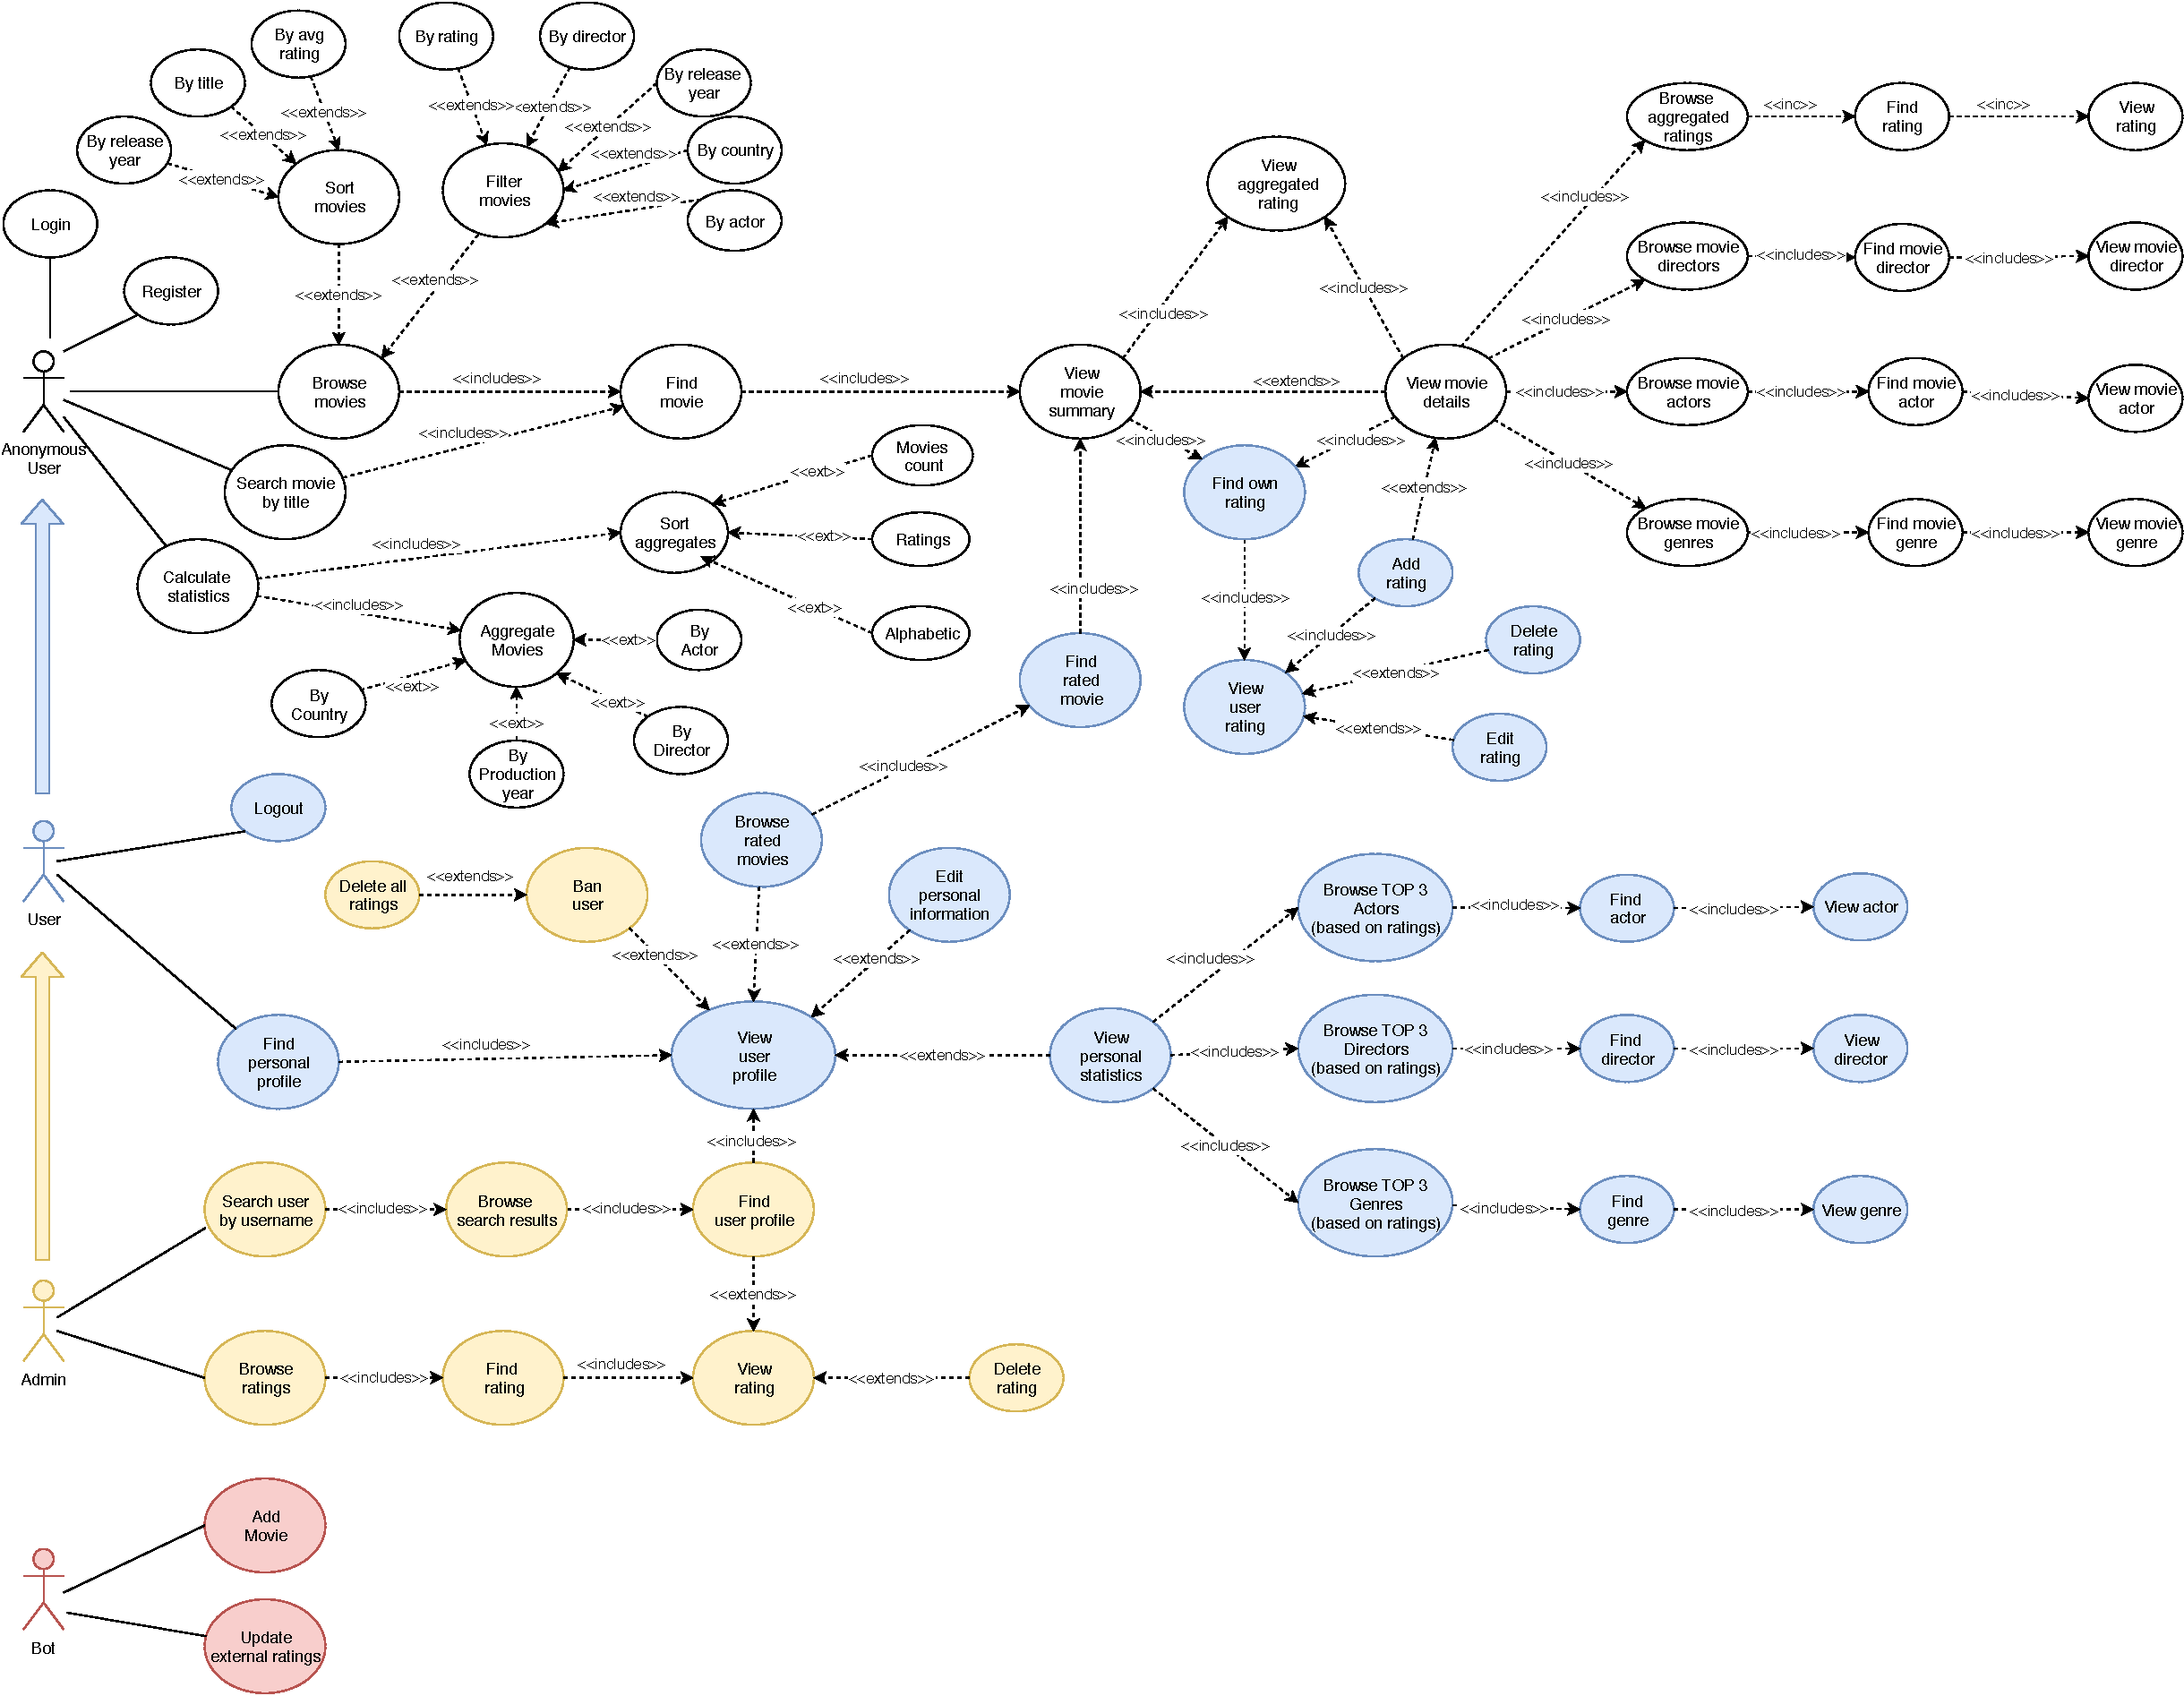
\includegraphics[height=18cm]{figs/use_case.pdf}
    \caption{Use-case diagram}
    \label{fig:usecase}
\end{sidewaysfigure}

The use-case diagram is shown in \cref{fig:usecase}. Different colors are used to highlight cases that are exclusive of some actors: white cases are referred to all users; blue and green cases are referred to registered user and admin; yellow cases are exclusive of the admin. Green cases highlight the ones that 
were introduced in task 3 and all refer to actions that a registered user can
do.

\subsection{Class diagram}

\begin{figure}[h!]
    \centering
    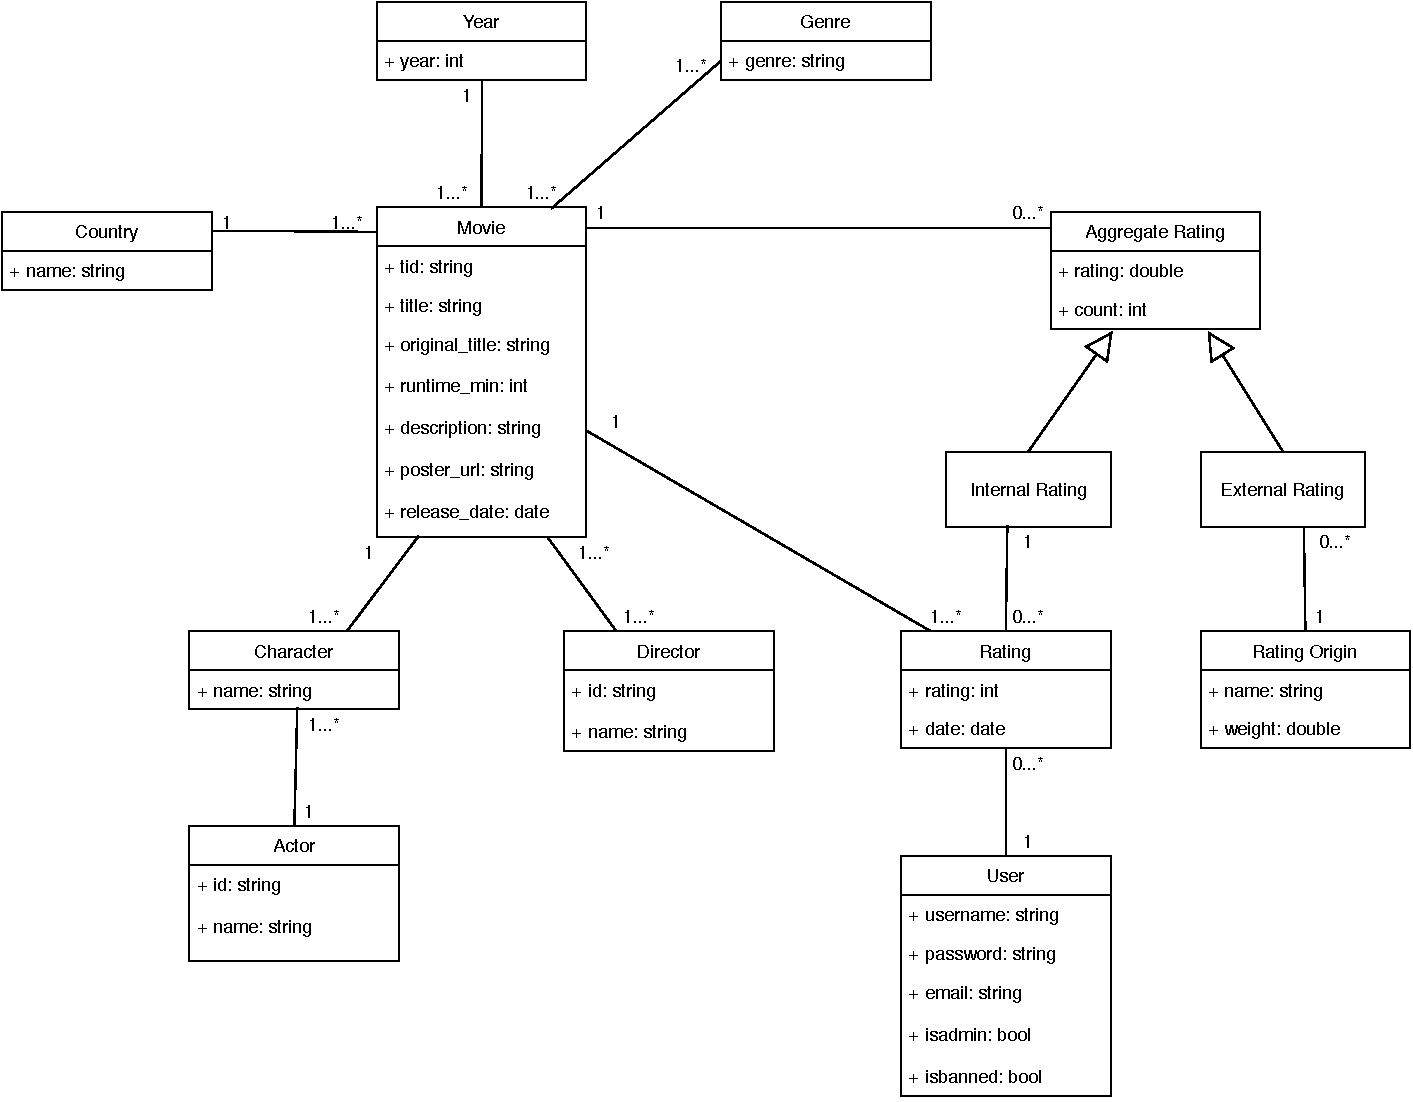
\includegraphics[width=\textwidth]{figs/class_diagram.pdf}
    \caption{Class diagram for the identified entities}
    \label{fig:class_diagram}
\end{figure}

The class diagram is shown in \cref{fig:class_diagram}. It was decided to show \emph{Country}, \emph{Year} and \emph{Genre} as separate entities as they are some of the fields over which aggregate statistics are calculated.

% ------------------------------------------------------------------------------

\clearpage
\subsection{Data model}
\begin{figure}[h!]
    \centering
    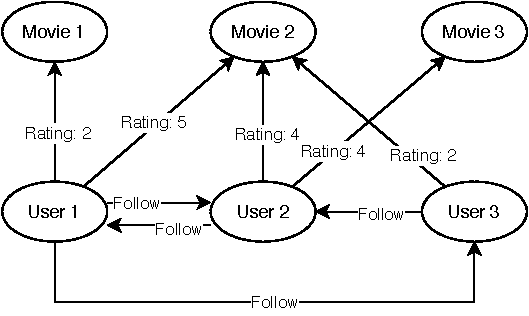
\includegraphics[width=.7\textwidth]{figs/graph_example.pdf}
    \caption{Example graph}
    \label{fig:graph_example}
\end{figure}
The graph database will have 2 different types of nodes and 2 types of edges:
\paragraph{Node types}
\begin{itemize}
	\item \textbf{Movie}: it will contain all information needed to show a list
		of suggested movies: \emph{id}, \emph{title}, \emph{year}, 
		\emph{poster}.
    \item \textbf{User}: it will contain only the \emph{username} and the \emph{\_id} since no other information is required.
\end{itemize}
\paragraph{Edge types}
\begin{itemize}
	\item \textbf{Rating} (User->Movie): it will contain the \emph{rating} as 
		attribute.
	\item \textbf{Follow} (User->User): no attribute is required.
\end{itemize}
In each following subsection, an example document is shown for every collection.

\subsection{Graph-centric operations}
This section will explain how we intend to execute the queries in the database in terms of graph operations. Simple CRUD operations will not be reported for brevity's sake.

\paragraph{Movie suggestion}
Movie will be suggested based on the ratings that users that liked similar 
movies as the user. For example, in figure \ref{fig:graph_example}, 
\emph{Movie 3} may be suggested to \emph{User 1} since \emph{User 2} liked 
\emph{Movie 2} as \emph{User 1} and he also liked \emph{Movie 3}. 
In practice, starting from a user we will go to each movie he
liked, then to the users who recently liked that movie, then to other movies 
they liked. We will then count the number of paths like the one described 
for each movie (the last one in the path) and show the user the top-N movies 
given this metric.

\paragraph{User suggestion}
Users to follow will be suggested based on the number of common follow 
relationships. For example, in figure \ref{fig:graph_example}, \emph{User 3}
may be suggested to \emph{User 2} since \emph{User 2} follows \emph{User 1}
that follows \emph{User 3}. In practice, starting from the user, we will go to
each user he follows and from here to each user that the latter user follows. 
We will then count the number of paths from the user to the users with common 
followers and show the user the top-N users given this metric.

\subsection{Software Architecture}

The application will be made of the following 4 components:
\begin{itemize}
	\item \textbf{Mongo DB}: a MongoDB cluster will be deployed with
		replication.
	\item \textbf{Neo4j}: an auxiliary graph database will be used to 	
		calculate more efficiently the movie suggestions and to store 
        information about follow relationships since this kind of operations
        are more suited to this kind of DB.
	\item \textbf{React Front-end}: web-based UI.
	\item \textbf{Java Back-end}: using \emph{Spring}, the \emph{Java back-end} will provide REST APIs to the \emph{React front-end}.
	\item \textbf{Updater ``bot''}: three Python scripts are needed in order to nightly update the DB with the latest movies and ratings: 
	\begin{enumerate}
		\item the \textbf{IMDB parser} periodically parses the IMDb dataset to add the latest movies.
		\item the \textbf{scraper} continuously parses the rating sources to update the ratings.
		\item the \textbf{synchronizer} periodically synchronizes movies from MongoDB to Neo4j.
	\end{enumerate}
	These scripts will executes asynchronously from the \emph{Java back-end}.
\end{itemize}
\end{document}